%------------------------------------------------

\begin{fullwidth}

% Intro ----------------------------------------

% Motivation
Transforming raw data into an academic manuscript,
a policy recommendation, a dashboard, a brief, or a report
requires a mix of subject expertise, programming skills,
and statistical and econometric knowledge.
In this chapter, we discuss the process of transforming
cleaned raw data into the final analysis dataset(s).
The process of data analysis is typically
a back-and-forth discussion between people
with differing skill sets.
An essential part of the process is translating the
raw data into economically meaningful indicators.
To effectively do this in a team environment,
data, code and outputs must be well-organized,
with a clear system for version control,
and analysis scripts structured such that any member of the research team can run them.
Putting in time upfront to structure the data analysis workflow
in this way pays substantial dividends throughout the process.

% Chapter overview
In this chapter, we suggest an a data analysis workflow
starting from clean raw data.
The first step is variable construction:
creating the actual outcomes of interest for analysis.
We emphasize the importance of transparently documenting research decisions
made in this process.
The second step is the analysis itself.
We do not offer instructions on how to conduct specific analyses,
as that is determined by research design,
and there are many excellent existing guides.
Rather, we discuss how to structure analysis code
so that it is easy to follow and understand,
for both the full research team members and a public audience.
Finally, we discuss ways to automate common outputs
so that your work is fully reproducible.

\end{fullwidth}

%------------------------------------------------

\section{Creating analysis datasets}

% What is construction
For this chapter, we assume you are starting from
one or multiple well-documented tidy\cite{hadley2017R} datasets.
We also assume that these datasets
have gone through thorough quality checks
and incorporate any corrections needed.
The next step is to \textbf{construct}\sidenote{
	\textbf{Data construction}:
	The process of transforming cleaned data into analysis data by
	creating the derived indicators that will be analyzed.}
the variables that you will use for analysis;
that is, to transform the cleaned data into analysis-ready data.
It's possible the acquired data is ready for analysis,
but in most cases it needs to be prepared by integrating different datasets
and creating derived variables
(dummies, indices, and interactions, to name a few\sidenote{
  See \citet{adjognon2019reducing} for an example.}).
The derived indicators you will construct should be
planned during research design\index{Research design};
the pre-analysis plan should serve as your guide
at this stage.\index{pre-analysis plan}
During construction, data will typically be
reshaped, merged, and aggregated to change the level of the data points
from the \textbf{unit of \textit{observation}} in the raw data
to the \textbf{unit of \textit{analysis}}.\sidenote{\url{
		https://dimewiki.worldbank.org/Unit\_of\_Observation}}\index{unit of observation}\index{unit of analysis}

% A project may require multiple purpose-built data sets
Each analysis dataset is built to answer an analysis question.
If the sub-samples and units of observation
vary for different pieces of the analysis,
you may need to create many purpose-built analysis datasets.\index{analysis datasets}
In such cases, it is not good practice
to try to create a single ``canonical'' analysis dataset.
For a concrete example of what this means,
think of an agricultural intervention
that was randomized across villages
and only affected certain plots within each village.
The research team may want to
run household-level regressions on income,
test for plot-level productivity gains,
and check if village characteristics are balanced.
Having three separate datasets for each of these three pieces of analysis
will result in cleaner, more efficient, and less error-prone analytical code than if
you started from a single analysis dataset and repeatedly transformed it.

\subsection{Fitting construction into the data workflow}

% Why construction is separate from data cleaning
Construction follows data cleaning and
should be treated as a separate task for two reasons.
First, this helps to clearly differentiate error corrections
(necessary for all data uses)
from creation of analysis indicators
(necessary only for specific analyses).
Second, it helps to ensure that variable definitions are
consistent across datasets.
Construction can create many outputs combining many inputs,
and, unlike in data cleaning,
resulting datasets should be concise rather than exhaustive.
For example, take a project that has a baseline and an endline survey.
Unless the two data collection instruments are exactly the same,
which is preferable but often not the case,
the data cleaning for each of these rounds will require different steps,
and therefore will be done separately.
However, the analysis indicators must be constructed in the exact same way,
so they are comparable.
To do this, you will require at least two separate cleaning scripts,
and a unified construction script.
Maintaining one construction script guarantees that you will not
accidentally make changes to an indicator from one round
while forgetting to update the other.

% Why construction is separate from analysis
When we visualize the research workflow,
variable construction precedes data analysis,
as derivative variables need to be created before they are analyzed.
In practice, however, as you analyze the data,
it is often useful to revisit construction,
and explore different subsets of the same and other transformations of the data.
Even if construction and analysis are done concurrently,
you should always do the two in separate scripts.
If every script that creates a table starts by loading a dataset,
subsetting it, and manipulating variables,
any edits to construction need to be replicated in all scripts.
This increases the chances that at least one of them
will have a different sample or variable definition.
Doing all variable construction and data transformation
in a unified script, separate from the analysis code, helps
avoid this and ensures consistency across different outputs.

\subsection{Integrating different data sources}

% When merging is necessary and how to start thinking about it
To create the analysis dataset,
it is typically necessary to combine or merge information
from different data sources.\sidenote{
	\url{https://dimewiki.worldbank.org/Data_Integration}}
For example, you may merge administrative data with survey data
in order to include demographic information in your analysis,
or you may want to integrate geographic information
in order to include location-specific controls.\sidenote{Such
	operations are commonly called ``merges'' in Stata, and
	``joins'' in R's \texttt{tidyverse} dialect.
	We will use the first term on the next few paragraphs.}
To understand how to perform such operations,
you will need to consider the unit of observation for each dataset,
and their respective identifying variables.
Merges are frequent and complex operations,
which makes them a common source of error.
Whichever statistical software you are using,
take the time to read through the help file of merge commands
and make sure you understand their options and outputs.\index{merging data}

% How to think about merges
Chapter 3 discussed how to merge datasets
based on their units of observation and identifying variables.
When writing the code to implement merge operations,
a few steps can help avoid mistakes.
First, before writing code to combine the datasets,
write pseudocode to understand which observations you expect to be
matched or not, and why.
When possible, determine exactly which and how many
matched and unmatched observations should result from the merge.
Second, think carefully about whether you want to keep matched and unmatched observations,
or only specific matching outcomes (e.g. to create a balanced panel),
and add that to the pseudocode as well.
Finally, run the code to merge the datasets,
and compare outcome to your expectations.
Add comments to explain any exceptions,
and make it so the code will return an error in case unexpected results show up in future runs.

% Common mistakes
To avoid unintentional changes to your data,
pay close attention to merge results.
Two issues to pay extra attention to are missing values and dropped observations.
Make sure to read about how each command treats missing observations:
are unmatched observations dropped, or are they kept with missing values?
Whenever possible, add automated checks in the script that throw an error message
if the result is different than what you expect,
or you may not changes in the outcome running large portions of code.
Document changes in the number of observations in your comments,
and explain why they are happening.
If your are subsetting your data by keeping only matched observations,
write down the reason why the observation differ across datasets,
as well as why you are only interested in those that matched.
The same applies when you are adding new observations from the merged dataset.

% Data integration
Some merges of data with different units of observation
are more conceptually complex.
Examples include: overlaying road location data with household data,
using a spatial match; combining school administrative data, such as attendance records and test scores,
with student demographic characteristics from a survey;
or linking a dataset of infrastructure access points, such as water pumps or schools,
with a dataset of household locations.
In these cases, a key part of the research contribution is figuring out
a useful way to combine the datasets.
Since the conceptual constructs that link observations from the two data sources
are important and can take many possible forms,
it is especially important for the data integration to not be treated mechanically,
and to be extensively documented, separately from other data construction tasks.


\subsection{Creating analysis variables}

% Main points to keep in mind for new variables
Once you have assembled variables from different sources into a single working dataset
with the right raw information and observations,
it's time to create the derived indicators of interest for analysis.\index{analysis variables}
Before constructing new indicators,
you must check and double-check units, scales, and value assignments of each variable that will be used.
This is when you will use the knowledge
of the data and the documentation developed during cleaning the most.
First, check that all categorical variables have the same value assignment,
such that labels and levels have the same correspondence across variables that use the same options.
For example, it's possible that in one question \texttt{0} means ``no'' and \texttt{1} means ``yes'',
while in another one the same answers were coded as \texttt{1} and \texttt{2}.\index{binary variables}
(We recommend coding binary questions as either \texttt{1} and \texttt{0} or \texttt{TRUE} and \texttt{FALSE},
so they can be used numerically as frequencies in means and as dummies in regressions.
This often implies re-expressing categorical variables like \texttt{gender} as binary variables like \texttt{woman}.)
Second, make sure that any numeric variables you are comparing
are converted to the same scale or unit of measure:
you cannot add one hectare and two acres and get a meaningful number.
New variables should be assigned functional names,
and the dataset ordered such that related variables are together.
Adding notes to each variable will make your dataset more user-friendly.

% Dealing with outliers and missing values
At this point, you will also need to decide
how to handle any outliers or unusual values identified during data cleaning.
How to treat outliers is a research question.\sidenote{
	\url{https://dimewiki.worldbank.org/Variable_Construction\#Dealing_with_outliers}}\index{outliers}
There are multiple possible approaches,
and the best choice for a particular case
will depend on the objectives of the analysis.
Whatever your team decides, make sure to explicitly note
what the decision was and how it was made.
Results can be sensitive to the treatment of outliers,
so keeping the original variable in the dataset
will allow you to test how much it affects your outputs.
All these points also apply to imputation of missing values and other distributional patterns.
As a general rule, never overwrite or delete original data during the construction process.
Always create derived indicators with new names.

% Maintaining indicator definition across rounds
Finally, creating a panel with survey data involves additional timing complexities.
It is common to construct indicators soon after receiving data from a new survey round.
However, creating indicators for each round separately increases the risk of using different definitions each time.
Having a well-established definition for each constructed variable helps prevent that mistake,
but the best way to guarantee it won't happen is to create the indicators for all rounds in the same script.
Say you constructed some analysis variables after baseline, and are now receiving midline data.
Then the first thing you should do is create a cleaned panel dataset,
ignoring the previous constructed version of the baseline data.
Our team created \texttt{iefieldkit}'s \texttt{iecodebook append} subcommand
% to-do % -----------------------------------------------------------------
% \sidenote{\url{STATA JORUNAL ARTICLE}}
% -------------------------------------------------------------------------
to help you reconcile and append data from cleaned survey rounds
or similar data collected from different contexts.\index{\texttt{iefieldkit}}\index{\texttt{iecodebook}}
This is done by completing an Excel sheet to indicate what changes in
names, value assignments, and value labels should be made so the data is consistent across rounds or settings.\sidenote{
  See \citet{daniels2017use} for an example.}
By doing so, you are also creating helpful documentation about your data work.
% to-do % --------------------------------------------------------
% See XXX for an example of a Stata do-file uses iecodebook append
% ----------------------------------------------------------------
Once data tables are consistently appended,
adapt your construction script so it can be used on the complete panel dataset.
In addition to preventing inconsistencies and documenting your work,
this process will also save you time and give you an opportunity to review your original code.


\subsection{Documenting variable construction}

% Why documentation is important: transparency and reproducibility
Because data construction involves translating concrete observed data points
to measures of abstract concepts,
it is important to document exactly how each variable is derived or calculated.
Careful documentation is closely linked to the research principles discussed in the first chapter.
It makes research decisions transparent,
as anyone can read about how you defined each variable in your analysis,
and what was the reasoning behind these decisions.
By reading the documentation,
someone unfamiliar with the project should be able to understand the contents of the analysis datasets,
the steps taken to create them, and the decision-making process through your documentation.
Ideally, they should also be able reproduce your steps and recreate the constructed variables.
Therefore, documentation is an output of construction as relevant as the code and data,
and it is good practice for papers to have an accompanying data appendix
listing analysis variables and their definitions.

% How to document construction
The development of construction documentation is a good opportunity to have
a wider discussion with your team about creating protocols for variable definition,
which will guarantee that indicators are defined consistently across projects.
You must have a detailed account of how variables are created.
This will be implemented in your code, but you should still
add comments explaining in human language what you are doing and why.
This is a crucial step both to prevent mistakes and to guarantee transparency.
To make sure that these comments can be more easily navigated,
it is wise to start writing a variable dictionary as soon as you begin making changes to the data.\sidenote{
	See \citet{jones2019factor} for an example.}
Carefully record how specific variables have been combined, recoded, and scaled,
and refer to those records in the code.

% iecodebook export
The \texttt{iecodebook export} subcommand is
a good way to ensure you have easy-to-read documentation.
When all your final indicators have been created,
you can use the it to list all variables in the dataset in an Excel sheet.
You can then add the variable definitions to that file to create a concise metadata document.
Take this opportunity to review your notes and make sure that your code
is implementing exactly what is described in the documentation.
% to-do % --------------------------------------------------------
% See XXX for an example of a Stata do-file uses iecodebook append
% ----------------------------------------------------------------

%------------------------------------------------

\section{Writing data analysis code}

% Intro: this section focuses on data analysis CODE
After data is cleaned and indicators are constructed, you are ready to start analyzing the data.
\index{data analysis}
There are many existing resources for data analysis and statistical methods, such as
\textit{R for Data Science};\cite{hadley2017R}
\textit{A Practical Introduction to Stata};\cite{RePEc:gdm:wpaper:9412}
\textit{Mostly Harmless Econometrics};\cite{angrist2008mostly}
and \textit{Causal Inference: The Mixtape}.\cite{cunningham2018causal}
We focus on how to structure data analysis code and files, rather than how to conduct specific analyses.

\subsection{Organizing analysis code}

% Exploratory vs final data analysis
The analysis stage usually starts with a process we call \textbf{exploratory data analysis}.\index{exploratory data analysis}
This is when you are first looking for patterns in your data,
creating descriptive graphs and tables,
and trying different tests to understand your results.
It progresses into \textbf{final analysis} when your team starts to decide which are the ``main results'', or
those that will make it into a research output.
The way you deal with code and code outputs for exploratory and final analysis is different.
During the exploratory stage,
you will be tempted to write lots of analysis into one big, impressive, start-to-finish script.
While this is fine when you are writing your research stream of consciousness into code,
it leads to poor practices in the final code such as not clearing the workspace
and not loading a fresh dataset before each analysis task.

% Write independent analysis scripts
To avoid mistakes, it's important to take the time
to organize the code that you want to keep, that is,
the final analysis code, in an organized manner.
The result is a curated set of polished scripts that
will be part of a reproducibility package.\index{reproducibility package}
A well-organized analysis script starts with a completely fresh workspace
and, for each output it creates, explicitly loads data before analyzing it.
This setup encourages data manipulation to be done earlier in the workflow
(that is, in separate cleaning and construction scripts).
This also prevents the common problem of having analysis scripts
that depend on other analysis scripts being run before them.
Such dependencies tend to require manual instructions
for all necessary chunks of code to be run in the right order.
We encourage you to code each task so
it is completely independent of all other code,
except for the analysis master script.
You can go as far as coding every output in a separate script.

% Writing easy to read analysis code
There is nothing wrong with code files being short and simple.
In fact, analysis scripts should be as simple as possible,
so whoever is reading them can focus on the concepts, not the coding.
Research questions and statistical decisions should be incorporated explicitly in the code through comments,
and their implementation should be easy to detect from the way the code is written.
This includes clustering, sampling, and controlling for different variables, to name a few.
If you have multiple analysis datasets,
each of them should have a descriptive name about its sample and unit of observation.
As your team comes to a decision about model specification,
you can create functions and globals (or objects) in the master script to use across scripts.
This is a good way to make sure specifications are consistent throughout the analysis.
It also makes your code more dynamic,
as it's easy to update specifications and results
through a master file without changing every script.

% to-do % ------------------------------------------------------------------------
% Add example of how to automatize research decisions through globals or functions
% --------------------------------------------------------------------------------

% Naming analysis code
To accomplish this, you will need to make sure that you have an effective data management system,
including file naming, organization, and version control.
Just as for the analysis datasets,
you should name each of the individual analysis files descriptively.
Code files such as \path{spatial-diff-in-diff.do},
\path{matching-villages.R}, and \path{summary-statistics.py}
are clear indicators of what each file is doing, and allow you to find code quickly.
If you intend to numerically order the script files
to correspond to exhibits as they appear in a paper or report,
leave this to near publication time,
as you will constantly re-order them during data analysis.

\subsection{Visualizing data}

% Useful resources for data visualization
\textbf{Data visualization}\sidenote{\url{
		https://dimewiki.worldbank.org/Data\_visualization}}\index{data visualization}
is increasingly popular,
and is becoming a field in its own right.\cite{healy2018data,wilke2019fundamentals}
Whole books have been written on how to create good data visualizations,
so we will not attempt to give you advice on it.
Rather, here are a few resources we have found useful.
The Tapestry conference focuses on ``storytelling with data''.\sidenote{
	\url{http://www.tapestryconference.com}}
\textit{Fundamentals of Data Visualization} provides extensive details on practical application;\sidenote{
	\url{https://serialmentor.com/dataviz}}
as does \textit{Data Visualization: A Practical Introduction}.\sidenote{
	\url{http://socvis.co}}
Graphics tools in Stata are highly customizable.
There is a fair amount of learning curve associated with
extremely-fine-grained adjustment,
but it is well worth reviewing the graphics manual.\sidenote{\url{
		https://www.stata.com/manuals/g.pdf}}
For an easier way around it,
you can use built-in and user-written graph schemes.\sidenote{
	\url{https://dimewiki.worldbank.org/Data_visualization}}
If you are an R user, the \textit{R Graphics Cookbook}
is a great resource for the its popular visualization package \texttt{ggplot}\sidenote{
	\url{https://r-graphics.org} and
	\url{https://ggplot2.tidyverse.org}}.
But there are a variety of other visualization packages,
such as \texttt{highcharter}, \texttt{r2d3}, \texttt{leaflet},
and \texttt{plotly} to name a few.\sidenote{
	\url{http://jkunst.com/highcharter},
	\url{https://rstudio.github.io/r2d3},
	\url{https://rstudio.github.io/leaflet} and
	\url{https://plot.ly/r}}
We have no intention of creating an exhaustive list,
but these are good places to start.\sidenote{
  \url{https://dimewiki.worldbank.org/Checklist:\_Reviewing\_Graphs}}

% Writing data viz code
We attribute some of the difficulty of creating good data visualization
to the difficulty of writing code to create them.
Making a visually compelling graph would already be hard enough if
you didn't have to go through many rounds of searching and reading help files 
to understand a command's graphical options syntax.
The trickiest part of using plotting commands is getting the data into the right format.
Though both Stata and R have plotting functions that graph summary statistics,
a good rule of thumb is to ensure that each
observation in your dataset corresponds to one data point in your desired visualization.
This may seem simple,
but often requires the aggregation and reshaping operations
discussed earlier in this chapter.

% Stata Visual Library and ietoolkit
Based on DIME's accumulated experience creating visualizations for impact evaluations,
our team has developed a few resources to facilitate this workflow.
First of all, we maintain a \textbf{Stata Visual Library}\sidenote{
	\url{https://worldbank.github.io/Stata-IE-Visual-Library}},
which has examples of graphs created in Stata and curated by us.\sidenote{
	A similar resource for R is \textit{The R Graph Gallery}: \url{https://www.r-graph-gallery.com}}
The Stata Visual Library includes example datasets to use with each do-file,
so you get a good sense of what your data should look like
before you can start writing code to create a visualization.
The \texttt{ietoolkit} package also contains two commands to automate
common impact evaluation graphs:
\texttt{iegraph} plots the values of coefficients for treatment dummies,
and \texttt{iekdensity} displays the distribution of an outcome variable
across groups and adds the treatment effect as a note.


%-------------------------------------------------------------------------
\section{Creating analysis outputs}

% Intro: why to think about outputs ahead of time
A great number of outputs will be created during the course of a project.
These will include both raw outputs such as tables and graphs
and final products such as presentations, papers and reports.
During exploratory analysis, your team will consider different approaches
to answer research questions and present answers.
Though it is best to be transparent about different
specifications tried and tests performed,
only a few will ultimately be considered ``main results''.
These will be \textbf{exported}\sidenote{
  \textbf{Exporting results:} The creation of publication-ready representations of results.}\index{exporting results} 
from the statistical software.
That is, they will be saved as tables and figures in format that is easier to interact with.
For example, saving graphs as images will allow your team to quickly see them,
as well as to add them as exhibits to other documents.
When the first of these code outputs are being created, agree on where to store them,
what software and formats to use, and how to keep track of them.
This discussion will save you time and efforts on two fronts:
you will spend less time formatting and polishing tables and graphs that
will not make their way into final research products;
and you will remember the different paths your team has already
taken, so you don't do the same thing twice.
This section will take you through key elements to keep in mind
when making workflow decisions and outputting results.


\subsection{Managing outputs}

% Where to store outputs
Decisions about storage of outputs are limited by technical constraints,
and dependent on file format.
Plain text formats like \texttt{.tex} and \texttt{.csv}
and should be managed through version control systems like Git,
as discussed in Chapter 2.
Binary outputs like Excel files, PDFs, PowerPoints, or Word documents,
on the other hand, should be kept in a synced folder.
Exporting all raw outputs as plain text files,
which can be done through all statistical software,
facilitates the identification of changes in results.
When you re-run your code from the master script,
the outputs will be overwritten,
and any changes (for example, in coefficients or number of observations)
will be automatically flagged for you or a reviewer to check.
Tracking changes to binary files is more cumbersome.
They they use more space,
which may cause slow down the cloud syncing.
There may be exceptions to this general rule
depending on the Git client you are using.
GitHub Desktop, for example,
displays changes in common binary image formats such as PNG files
in an accessible manner.

% Tracking scripts and their outputs
You will need to update your outputs frequently.
And if you have tried to recreate a result after a few months,
you probably know that it can be hard to remember where the code that created it was saved.
File naming conventions and code organization,
including easily searchable file names and comments,
play a key role in not re-writing scripts again and again.
We recommend maintaining one ``final'' analysis folder
and one folder with draft code or exploratory analysis.
The latter contains pieces of code that are stored for reference,
but not cleaned up to be included in any final outputs.
Once an output presents a result in the clearest manner possible,
it should be renamed and moved to the ``final analysis'' folder.
It's typically desirable to have the names of outputs and scripts linked --
so, for example, \texttt{factor-analysis.do} creates \texttt{factor-analysis.eps} and so on.
Document output creation in the master script that runs your code,
so that before the line that runs a particular analysis script
there are a few lines of comments listing
datasets and functions that are necessary for it to run,
as well as all outputs created by that script.

% to-do % ----------------------
% Add an example analysis master
% ------------------------------

% File formats
Knowing how your code outputs will be used will help you decide the best format to export them.
You can often save figures into different formats,
such as \texttt{.eps}, \texttt{.png}, \texttt{.pdf} or \texttt{.jpg}.
However, the decision between using Office Suite software such as Word and Power Point
versus {\LaTeX} and other plain text formats may influence how you write your code,
as this choice often implicates in the use of a particular command.
We strongly recommend that you chose software to create final products
that can be linked to raw outputs in such a way that they are updated
in the paper or presentation every time changes are made to them.
We broadly call files that have this feature \textbf{dynamic documents},\index{dynamic documents}
and they will be discussed in more detail in the final section of this chapter.


\subsection{Exporting analysis outputs}

% Which outputs should be fully automated and why
As briefly discussed in the previous section,
you do not necessarily have to export each and every table and graph
created during exploratory analysis.
Most statistical software allow you to review results interactively,
and this is often preferred at this stage.
Final analysis scripts, on the other hand, must export outputs
that are ready to be included in a paper or report.
No manual edits, including formatting,
should be necessary after exporting final outputs.
Manual edits are difficult to reproduce;
the less you make, the more reproducible your output is.
You may think that it's not worth coding a small formatting adjustment,
but you will inevitably need to make changes to the output,
and automating them will save you time by the end of the process.
(However, don't spend much time formatting tables and graphs until
you have come to a decision about which will be used for your final product.\sidenote{
	For a more detailed discussion on this, including different ways to export tables from Stata,
	see \url{https://blogs.worldbank.org/impactevaluations/nice-and-fast-tables-stata}})
Polishing final outputs can be a time-consuming process,
and you want to do it as few times as possible.

% Don't copy-paste!!
We cannot stress this enough:
do not set up a workflow that requires copying and pasting results.
Copying results from Excel to Word is error-prone and inefficient.
Copying results from a software console is risk-prone,
even more inefficient, and totally unnecessary.
The amount of work needed in a copy-paste workflow increases
rapidly with the number of tables and figures included in a research output,
and so do the chances of having the wrong version of a result in a paper or report.

% Output formats
There are numerous commands to export outputs from both R and Stata.
Some examples are \texttt{estout},\cite{estout05, estout07}
\texttt{outreg2},\cite{wada2014outreg2}
and \texttt{outwrite}\cite{daniels2019outwrite} in Stata,
and \texttt{stargazer}\cite{hlavac2015stargazer}
and \texttt{ggsave}\sidenote{\url{https://ggplot2.tidyverse.org/reference/ggsave.html}} in R.
They allow for a wide variety of output formats. We recommend using formats that are accessible and, whenever possible, lightweight.
Accessible means that it's easy for other people to open them.
In Stata, that would mean always using \texttt{graph export} to save images as
\texttt{.jpg}, \texttt{.png}, \texttt{.pdf}, etc.,
instead of \texttt{graph save},
which creates a \texttt{.gph} file that can only be opened by Stata.
Some publications require ``lossless'' TIFF or EPS files,
which are created by specifying the desired extension.
Whichever format you decide to use,
remember to always specify the file extension explicitly.
For tables, there are fewer file format options.
Given our recommendation to use \textbf{dynamic documents},\index{dynamic documents}
which will be discussed in more detail both in the next section and in Chapter 7,
exporting tables to \texttt{.tex} is preferred.
Excel \texttt{.xlsx} and \texttt{.csv} are also commonly used,
but often require the extra step of copying the tables into the final output.
The \texttt{ietoolkit} package includes two commands to export formatted tables,
automating the creation of common outputs and saving time for research.\index{\texttt{ietoolkit}}
\texttt{iebaltab}\sidenote{\url{https://dimewiki.worldbank.org/iebaltab}}
creates and exports balance tables to Excel or {\LaTeX}.\index{{\LaTeX}}
\texttt{ieddtab}\sidenote{\url{https://dimewiki.worldbank.org/ieddtab}}
does the same for difference-in-differences regressions.

% Last touches: formatting tables and including meta data
If you need to create a table with a very specific format
that is not automated by any command you know, consider writing it manually
(Stata's \texttt{filewrite} and R's \texttt{cat()}, for example, allow you to do that).
This will allow you to write a cleaner script that focuses on the econometrics,
and not on complicated commands to create and append intermediate matrices.
Keep in mind that final outputs should be self-standing.
This means it should be easy to read and understand them with only the information they contain.
Make sure labels and notes cover all relevant information
included in your code and comments that are not otherwise visible in the output.
Examples of information that should be included in labels and notes include sample,
unit of observation, unit of measurement, and variable definition.\sidenote{
	\url{https://dimewiki.worldbank.org/Checklist:\_Submit\_Table}}

\section{Preparing dynamic documents}

% Intro: what it is and why to use it
\textbf{Dynamic documents}\sidenote{
  \textbf{Dynamic documents:} File types that include direct references
  to exported materials and update them in the output automatically.}\index{dynamic documents}
are a broad class of tools that enable a streamlined, reproducible workflow.
The term ``dynamic'' can refer to any document-creation technology
that allows the inclusion of explicitly encoded linkages to raw output files.
This means that, whenever outputs are updated,
the next time the document is loaded or compiled, it will automatically include
all changes made to all outputs without any additional intervention from the user.
This is not possible in tools like Microsoft Office,
although there are tools and add-ons that produce similar functionality.
In Word, by default, you have to copy and paste each object individually
whenever tables, graphs, or other inputs have to be updated.
This workflow becomes more complex as the number of inputs grows,
increasing the likelihood of making mistakes or missing updates.
Dynamic documents prevent this from happening by managing document compilation and
inclusion of inputs in a single integrated process,
so you can skip the copying and pasting altogether.

\subsection{Dynamic exploratory analysis}

% Markdown
If all team members working on a dynamic document are comfortable using the same statistical software,
built-in dynamic document engines are a good option for exploratory analysis.
With these tools,
you can write both text (often in Markdown\sidenote{\url{https://www.markdownguide.org/}}) and code in the script,
and the result will usually be a PDF or HTML file including code, text, and outputs.
In our experience, many researchers find the entry cost to learning how to use these tools to be high.
These types of dynamic document tools are typically best used by the team members working most closely with code,
and can be great for creating exploratory analysis reports as you work on them,
or paper appendices including large chunks of code and dynamically created graphs and tables.
RMarkdown\sidenote{\url{https://rmarkdown.rstudio.com}} is the most widely adopted solution in R.
Stata offers a built-in package for dynamic documents, \texttt{dyndoc},\sidenote{\url{
		https://www.stata.com/manuals/rptdyndoc.pdf}}
and user-written commands such as \texttt{markstat},\sidenote{\url{https://data.princeton.edu/stata/markdown}}
\texttt{webdoc},\sidenote{\url{http://repec.sowi.unibe.ch/stata/webdoc}} and
\texttt{texdoc}.\sidenote{\url{http://repec.sowi.unibe.ch/stata/texdoc}}
The advantage of these tools in comparison with LaTeX is that
they create full documents from within your scripts,
so running the code and compiling the document is reduced to a single step.

% Non-code options
Documents called ``notebooks''
(such as Jupyter Notebook\sidenote{\url{https://jupyter.org}})
work similarly,
as they also use the underlying code that create the document.
These tools are usually appropriate for short or informal documents
because it tends to be difficult for those who are not familiar with them to edit the content,
and they often don't offer as extensive formatting options as, for example, Word.
There are also other simple tools for dynamic documents
that do not require direct operation of the underlying code or software,
simply access to the updated outputs.
An example of this is Dropbox Paper,
a free online writing tool that can be linked to files in Dropbox
which are automatically updated anytime the file is replaced.
These have limited functionality in terms of version control and formatting,
and may never include any references to confidential data,
but they do offer extensive collaboration features,
and can be useful for working on informal outputs.
Markdown files on GitHub can also provide similar functionality through the browser,
and are version controlled.
However, as with other Markdown options, the need to learn a new syntax may
discourage take up among team members who don't work with GitHub more extensively.

\subsection{Using {\LaTeX} for dynamic research outputs}

% What is LaTeX
Though formatted text software such as Word and PowerPoint are still prevalent,
researchers are increasingly choosing to prepare final outputs
like documents and presentations using {\LaTeX}.\index{{\LaTeX}}
{\LaTeX} is a document preparation and typesetting system with a unique code syntax.\sidenote{See
	\url{https://www.latex-project.org} and \url{https://github.com/worldbank/DIME-LaTeX-Templates}.}
While {\LaTeX} has a significant learning curve,
its enormous flexibility in terms of operation, collaboration, output formatting, and styling
make it our preferred choice for most large technical outputs.
In fact, {\LaTeX} operates behind-the-scenes in many other dynamic document tools (discussed below).
Therefore, we recommend that you learn {\LaTeX} as soon as you are able to.

% Advantages of LaTeX
The main advantage of using {\LaTeX} is that it updates outputs every time the document is compiled,
while still allowing for text to be added
and extensively formatted to publication-quality standards.
Additionally, because of its popularity in the academic community,
social scientists are more familiar with it than other dynamic documents tools,
so the cost of entry for a team is often relatively low.
Because \texttt{.tex} files are plain text,
they can be version-controlled using Git.
Creating documents in {\LaTeX} using an integrated writing environment such as TeXstudio, TeXmaker or LyX
is great for outputs that focus mainly on text
and include figures and tables that may be updated.
It is good for adding small chunks of code into an output.
Finally, some journals make {\LaTeX} templates available,
so papers can be more easily be formatted into their specific layout.

\section{Looking ahead}

\begin{fullwidth}
	\begin{figure}
		\centering
		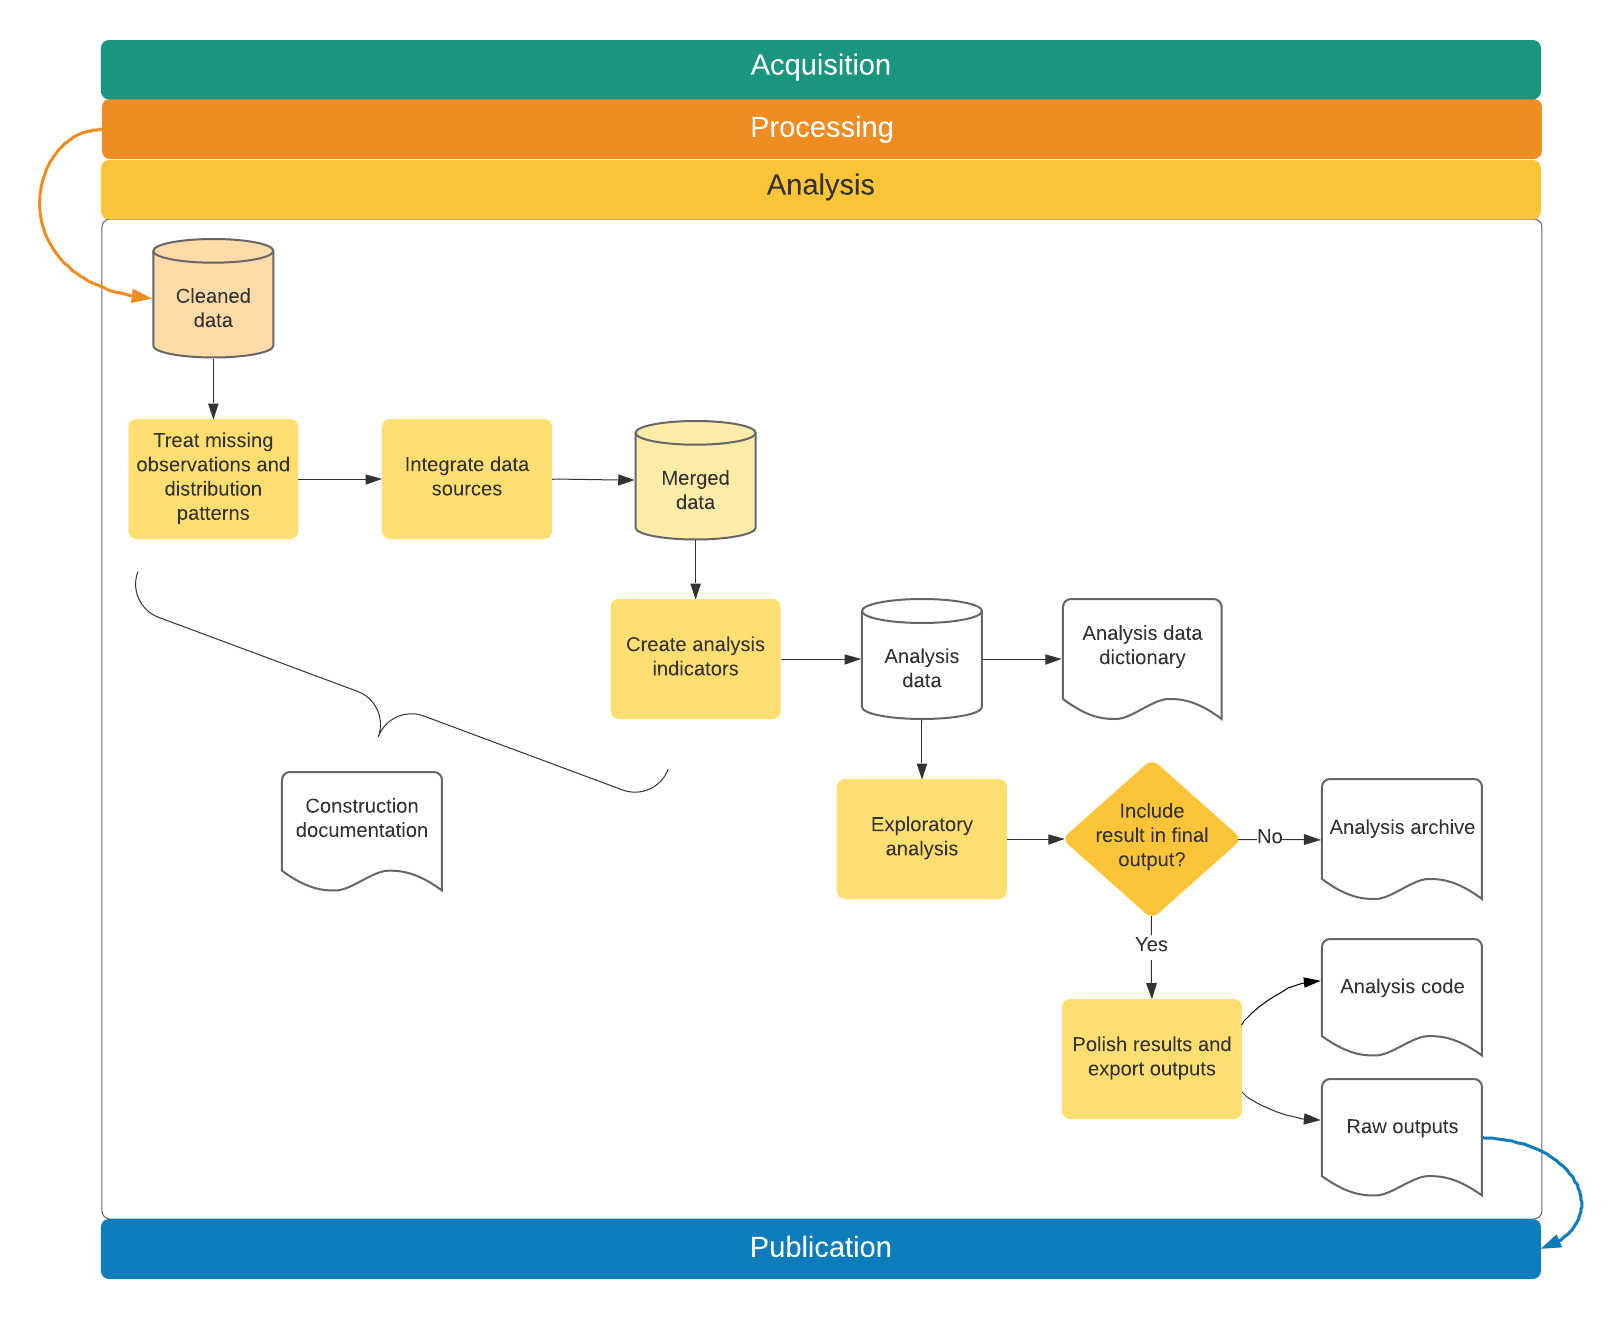
\includegraphics[width=1.6\linewidth]{diagrams/Analysis}
		\caption{Data analysis workflow}
		\label{fig:analysis}
	\end{figure}
\end{fullwidth}

%------------------------------------------------
